\documentclass[aspectratio=169]{beamer}

\usetheme[progressbar=frametitle]{metropolis}
\usepackage{appendixnumberbeamer}
\usepackage{booktabs}
\usepackage[scale=2]{ccicons}
\usepackage{xspace}
\usepackage{caption}
\usepackage{subcaption}
\usepackage{amsmath, amssymb}

\title{Лекция 9: Сверточные нейронные сети}
\date{11 апреля 2020}

\begin{document}

\maketitle

\begin{frame}{Полносвязная нейронная сеть}
    \centering
    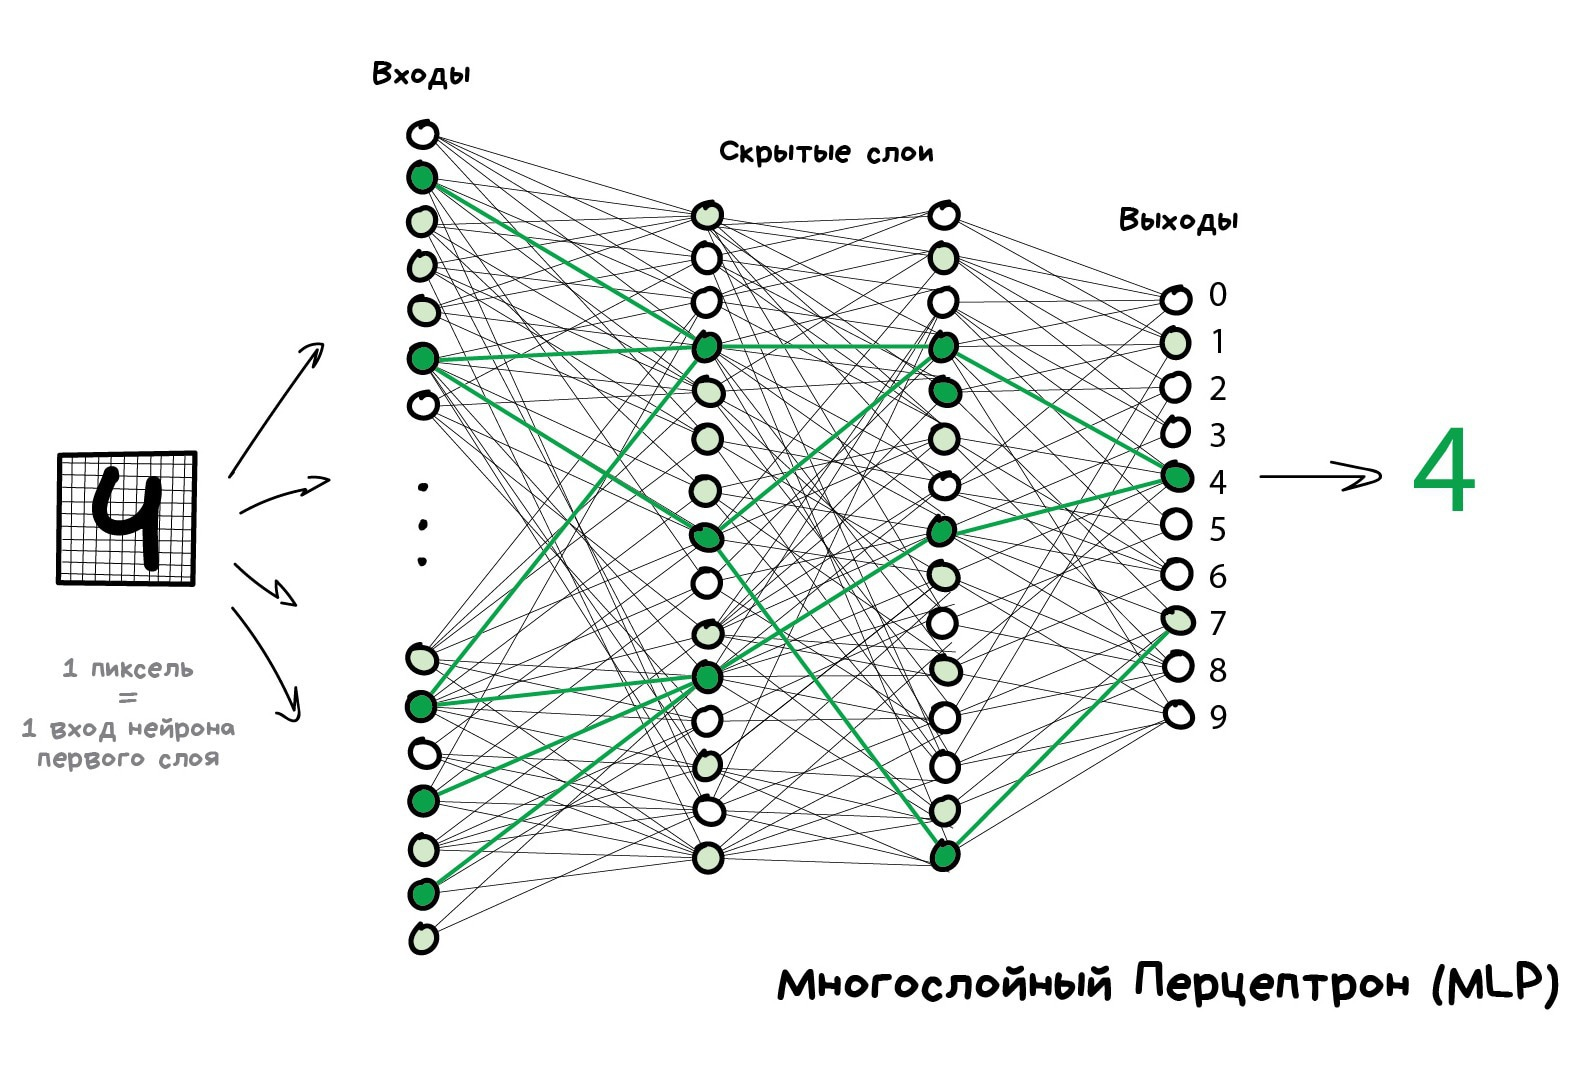
\includegraphics[width=0.7\linewidth]{graphs/four_layers.jpg}
\end{frame}

\begin{frame}{Сверточный оператор}
    \centering
    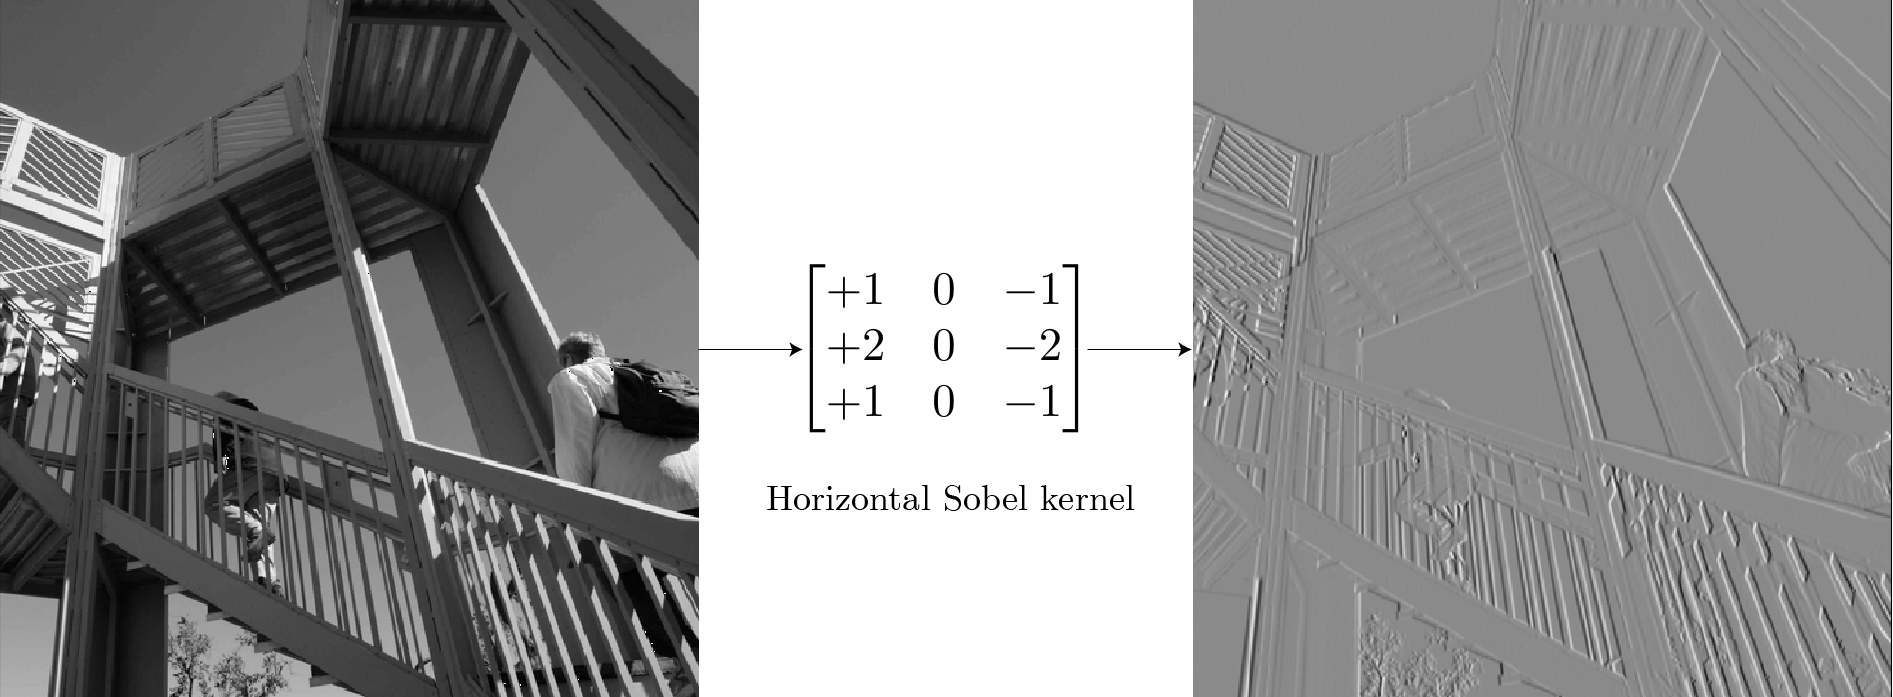
\includegraphics[width=\linewidth]{graphs/sobel.png}
\end{frame}

\begin{frame}{Сверточные фильтры}
    \centering
    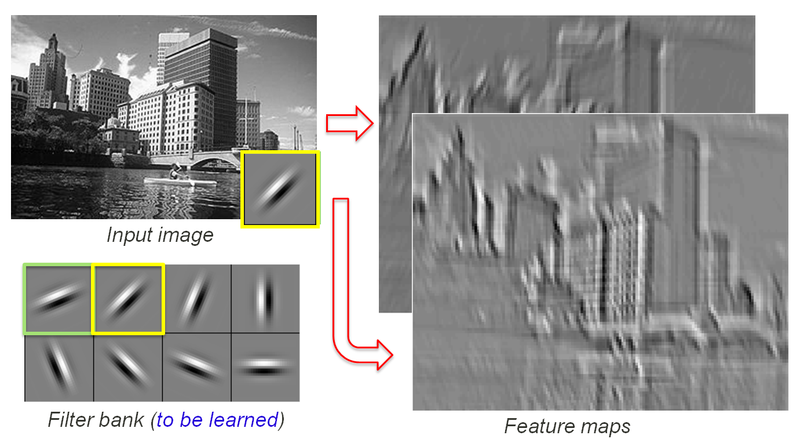
\includegraphics[width=0.85\linewidth]{graphs/conv_filter.png}
\end{frame}

\begin{frame}{Пулинг}
    \centering
    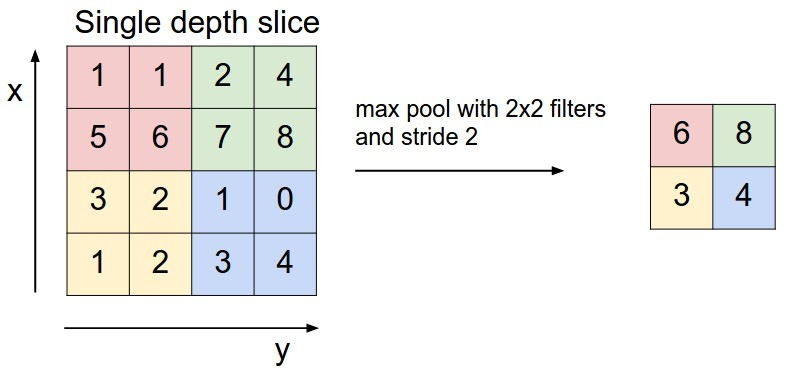
\includegraphics[width=\linewidth]{graphs/maxpool.jpeg}
\end{frame}

\begin{frame}{Структура простой CNN}
    \centering
    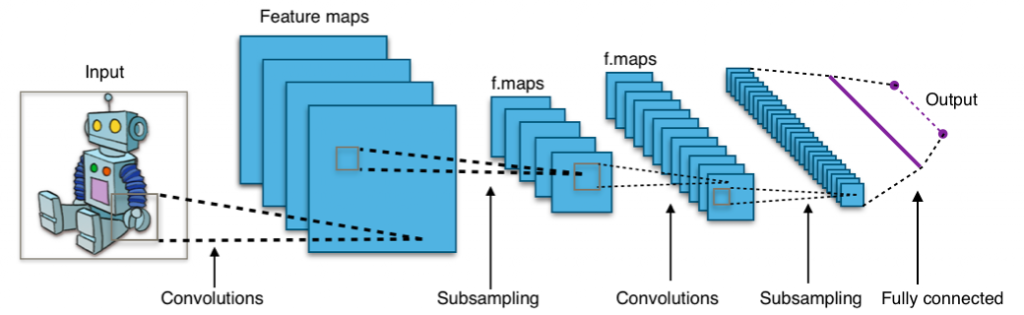
\includegraphics[width=0.63\linewidth]{graphs/typical_cnn.png}
    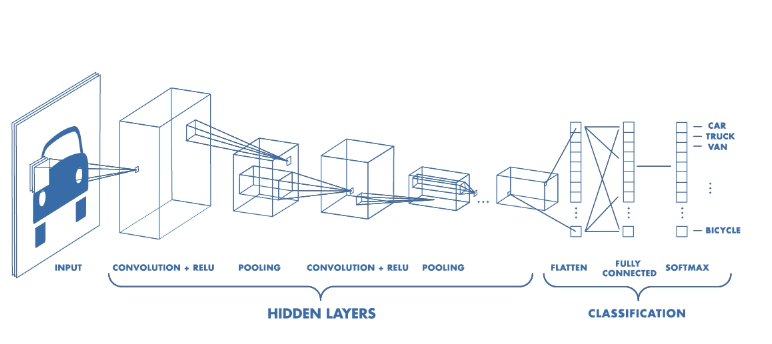
\includegraphics[width=0.63\linewidth]{graphs/typical_cnn2.png}
\end{frame}

\end{document}